% \section*{BÀI TẬP CUỐI CHƯƠNG IX}
\subsection{Bài tập trắc nghiệm tổng hợp}
\Opensolutionfile{ans}[ans/ans-KNTT-8.OTC]
\begin{ex} %[1K8BR-3]
	Một hộp đựng $20$ tấm thẻ cùng loại đánh số từ 1 đến 20. rút ngẫu nhiên một tấm thẻ trong hộp. Gọi $A$ là biến cố \lq\lq Rút được tấm thẻ ghi số chẵn lớn hơn $9$\rq\rq, $B$ là biến cố \lq\lq Rút được tấm thẻ ghi số không nhỏ hơn $8$ và không lớn hơn $15$\rq\rq. Số phần tử của $A\cup B$ là 
	\choice
	{\True$11$}
	{$10$}
	{$12$}
	{$13$}
	\loigiai{
	$A=\left\{10;12;14;16;18;20\right\}$; $B=\left\{8;9;10;11;12;13;14;15\right\}$.\\
	Suy ra $A\cup B=\left\{8;9;10;11;12;13;14;15;16;18;20\right\}$. \\
	Vậy $A\cup B$ có $11$ phần tử. }
\end{ex}
\begin{ex} %[1K8BR-3]
	Một hộp đựng $20$ tấm thẻ cùng loại đánh số từ 1 đến 20. rút ngẫu nhiên một tấm thẻ trong hộp. Gọi $A$ là biến cố \lq\lq Rút được tấm thẻ ghi số chẵn lớn hơn $9$\rq\rq, $B$ là biến cố \lq\lq Rút được tấm thẻ ghi số không nhỏ hơn $8$ và không lớn hơn $15$\rq\rq. Số phần tử của $AB$ là
	\choice
	{$5$}
	{$6$}
	{\True$3$}
	{$4$}
	\loigiai{
	$A=\left\{10;12;14;16;18;20\right\}$; $B=\left\{8;9;10;11;12;13;14;15\right\}$.\\
	Suy ra $A\cap B=\left\{10;12;14\right\}$.\\
	 Vậy $A B$ có $3$ phần tử.}
\end{ex}
\begin{ex} %[1K8BS-3]
	Tại một hội thảo quốc tế có $50$ nhà khoa học, trong đó có $31$ người thành thạo tiếng Anh, $21$ người thành thạo tiếng Pháp và $5$ người thành thạo cả tiếng Anh và tiếng Pháp. Chọn ngẫu nhiên một người trong hội thảo. Xác suất để người được chọn thành thạo ít nhất một trong hai thứ tiếng Anh hoặc Pháp là 
	\choice
	{\True$\dfrac{47}{50}$}
	{$\dfrac{37}{50}$}
	{$\dfrac{39}{50}$}
	{$\dfrac{41}{50}$}
	\loigiai{
	Gọi biến cố $A$ \lq\lq Người được chọn thành thạo tiếng An\rq\rq.\\
	Biến cố $B$ \lq\lq Người được chọn thành thạo tiếng Pháp\rq\rq.\\
	Biến cố $A\cup B$ \lq\lq Người được chọn thông thạo tiếng Anh hoặc tiếng Pháp\rq\rq\\
	Biến cố $AB$ \lq\lq Người được chọn thông thạo cả tiếng Anh và tiếng Pháp\rq\rq.
Khi đó 
$$P(A)=\frac{31}{50}; \ P(B)=\frac{21}{50};\ P(AB)=\frac{5}{50}.$$
Do đó, $P(A\cup B)=P(A)+P(B)-P(AB)=\dfrac{31}{50}+\dfrac{21}{50}-\dfrac{5}{50}=\dfrac{47}{50}$.}
\end{ex}
\begin{ex} %[1K8BS-3]
	Tại một hội thảo quốc tế có $50$ nhà khoa học, trong đó có $31$ người thành thạo tiếng Anh, $21$ người thành thạo tiếng Pháp và $5$ người thành thạo cả tiếng Anh và tiếng Pháp. Chọn ngẫu nhiên một người trong hội thảo. Xác suất để người được chọn không thông thạo cả hai thứ tiếng Anh hoặc Pháp là 
	\choice
	{$\dfrac{7}{50}$}
	{\True$\dfrac{3}{50}$}
	{$\dfrac{9}{50}$}
	{$\dfrac{11}{50}$}
	\loigiai{
	Gọi biến cố $C$ \lq\lq Người được chọn không thông thạo cả hai thứ tiếng Anh hoặc Pháp\rq\rq. Ta thấy, $C$ và $A\cup B$ là hai biến cố đối nhau. Do đó,
	$$P(C)=1-P(A\cup B)=1-\frac{47}{50}=\frac{3}{50}.$$}
\end{ex}
\begin{ex}%[1K8KT-4]
	Một lớp có $40$ học sinh, trông đó có $23$ học sinh thích bóng chuyền, $18$ học sinh thích bóng rổ, $26$ học sinh thích bóng chuyền hoặc bóng rổ hoặc cả hai. Chọn ngẫu nhiên một học sinh trong lớp. Xác suất để chọn được học sinh không thích cả bóng chuyền và bóng rổ là
	\choice
	{$\dfrac{18}{40}$} 
	{\True$\dfrac{14}{40}$} 
	{$\dfrac{19}{40}$} 
	{$\dfrac{21}{40}$}
	\loigiai{
	Gọi biến cố $A$ \lq\lq Học sinh được chọn thích bóng chuyển\rq\rq. \\
Biến cố $B$ \lq\lq Học sinh được chọn thích bóng rổ\rq\rq. Khi đó, ta có $$P(A)=\dfrac{23}{40};\ P(B)=\dfrac{18}{40}; \ P(A\cup B)=\dfrac{26}{40}.$$
Suy ra xác suất để chọn được học sinh không thích cả bóng chuyền và bóng rổ là
$$P(\bar{A}\bar{B})=1-P(A\cup B)=1-\dfrac{26}{40}=\dfrac{14}{40}.$$} 
\end{ex}
\begin{ex}%[1K8KT-4]
	Một lớp có $40$ học sinh, trông đó có $23$ học sinh thích bóng chuyền, $18$ học sinh thích bóng rổ, $26$ học sinh thích bóng chuyền hoặc bóng rổ hoặc cả hai. Chọn ngẫu nhiên một học sinh trong lớp. Xác suất để chọn được học sinh thích bóng chuyền và không thích bóng rổ là 
	\choice
	{$\dfrac{7}{40}$} 
	{$\dfrac{9}{40}$} 
	{\True$\dfrac{8}{40}$} 
	{$\dfrac{11}{40}$}
	\loigiai{
	Gọi biến cố $A$ \lq\lq Học sinh được chọn thích bóng chuyển\rq\rq. \\
	Biến cố $B$ \lq\lq Học sinh được chọn thích bóng rổ\rq\rq. Khi đó, ta có $$n(A)=23;\ n(B)=18; \ n(A\cup B)=26 \Rightarrow n(AB)=23+18-26=15.$$
	Suy ra $n(A\bar{B})=23-15=8.$ Vậy xác suất để chọn được học sinh thích bóng chuyền và không thích bóng rổ là 
	$$P(A\bar{B})=\dfrac{8}{40}.$$}
\end{ex}
%-----
\begin{ex}%[VU NGOC HAO]%[1T9Y1-1]
	Gieo $2$ con xúc xắc cân đối và đồng chất. Gọi $A$ là biến cố \lq\lq Tích số chấm xuất hiện là số lẻ\rq\rq. Biến cố nào sau đây xung khắc với biến cố $A$?
	\choice
	{\lq\lq Xuất hiện hai mặt có cùng số chấm\rq\rq}
	{\True \lq\lq Tổng số chấm xuất hiện là số lẻ\rq\rq}
	{\lq\lq Xuất hiện ít nhất một mặt có số chấm là số lẻ\rq\rq}
	{\lq\lq Xuất hiện hai mặt có số chấm khác nhau\rq\rq}
	\loigiai{
	Biến cố $A$: \lq\lq Tích số chấm xuất hiện là số lẻ\rq\rq\; tức là cả hai 
	mặt 
	xuất hiện đều là lẻ.\\
	Biến cố $B$: \lq\lq Tổng số chấm xuất hiện là số lẻ\rq\rq\; tức là một mặt 
	là 
	lẻ và một mặt là chẵn.\\
	Suy ra $A \cap B=\emptyset$. Vậy $A$ và $B$ là hai biến cố xung khắc.
	}
\end{ex}
\begin{ex}%[VU NGOC HAO]%[1T9Y2-3]
	Cho $A$ và $B$ là hai biến cố độc lập. Biết $P(A)=0{,}4$ và $P(B)=0{,}5$. Xác suất của biến cố $A \cup B$ là
	\choice
	{$0{,}9$ }
	{\True $0{,}7$} 
	{$0{,}5$} 
	{$0{,}2$}
	\loigiai{
	Ta có $P(A \cup B)=P(A)+P(B)-P(AB)=0{,}4+0{,}5-0{,}4 \cdot 0{,}5=0{,}7.$ 	
	}
\end{ex}
\begin{ex}%[VU NGOC HAO]%[1T9Y1-1]
	Gieo $2$ con xúc xắc cân đối và đồng chất. Xác suất của biến cố \lq\lq Tổng số chấm xuất hiện trên hai con xúc xắc chia hết cho $5$\rq\rq$\,$là
	\choice
	{$\dfrac{5}{36}$}
	{$\dfrac{1}{6}$}
	{\True $\dfrac{7}{36}$}
	{$\dfrac{2}{9}$}
	\loigiai{
	Ta có $n(\Omega)=6^2=36.$\\
	Gọi biến cố \lq\lq Tổng số chấm xuất hiện trên hai con xúc xắc chia hết cho $5$\rq\rq$\,$ nên \\$A= \{ (1;4), (4;1) (2;3), (3;2) (4;6), (6;4), (5;5)\} \Rightarrow 
	n(A)=7$.\\
	Vậy $P(A)=\dfrac{7}{36}$.
	}
\end{ex}
\begin{ex}%[VU NGOC HAO]%[1T9Y2-1]
	Lấy ra ngẫu nhiên $2$ quả bóng từ một hộp chứa $5$ quả bóng xanh và $4$ quả bóng đỏ có kích thước và khối lượng như nhau. Xác suất của biến cố \lq\lq Hai bóng lấy ra có cùng màu\rq\rq $\,$là
	\choice
	{$\dfrac{1}{9}$}
	{$\dfrac{2}{9}$}
	{\True $\dfrac{4}{9}$}
	{$\dfrac{5}{9}$}
	\loigiai{
	Ta có $n(\Omega)=\mathrm{C}_9^2=36.$\\
	$n(A)=\mathrm{C}_5^2 + \mathrm{C}_4^2=16$.\\
	Vậy $P(A)=\dfrac{16}{36}=\dfrac{4}{9}$.	
	}
\end{ex}
\begin{ex}%[VU NGOC HAO]%[1T9K1-1]
	Chọn ngẫu nhiên $2$ đỉnh của một hình bát giác đều nội tiếp trong đường 
	tròn tâm $O$ bán kính $R$. Xác suất để khoảng cách giữa hai đỉnh đó bằng 
	$R \sqrt{2}$ là
	\choice
	{\True $\dfrac{2}{7}$}
	{ $\dfrac{3}{7}$}
	{$\dfrac{4}{7}$}
	{$\dfrac{5}{56}$}
	\loigiai{
	\immini{
	Gọi X là biến cố: \lq\lq Chọn được 2 đỉnh mà khoảng cách giữa hai đỉnh 
	đó bằng $R \sqrt{2}$ \rq\rq.\\
	Ta có $n(\Omega)=\mathrm{C}_8^2=28.$\\
	$\widehat{AOB}=\widehat{BOC}=\widehat{COD}=\widehat{DOE}=\widehat{EOF}
	=\widehat{FOG}=\widehat{GOH}=\widehat{HOA}=45^\circ$.\\
	Xét tam giác $AOC$ vuông cân tại $O$ có $OA=OC=R\Rightarrow 
	AC=R\sqrt{2}$.\\
	Tương tự ta có $X=\{AC,BD,CE,DF,EG,FH,GA,HB\}\Rightarrow n(X)=8.$\\
	Vậy $P(X)=\dfrac{8}{28}=\dfrac{2}{7}$.
	}{
	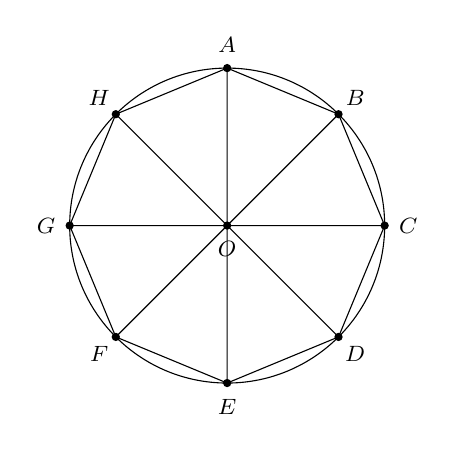
\begin{tikzpicture}[scale=1, font=\footnotesize, line join=round, 
	line cap=round, >=stealth]
	\def\r{2}
	\path 
	(0,0) coordinate (O)
	(90:\r) coordinate (A)
	(45:\r) coordinate (B)
	(0:\r) coordinate (C)
	(-45:\r) coordinate (D)
	(-90:\r) coordinate (E)
	(-135:\r) coordinate (F)
	(180:\r) coordinate (G)
	(135:\r) coordinate (H);
	\draw (O) circle (\r);
	\draw (A)--(B)--(C)--(D)--(E)--(F)--(G)--(H)--cycle
	(A)--(E) (B)--(F) (C)--(G) (H)--(D);
	\foreach \p/\r in 
	{O/-90,A/90,B/45,C/0,D/-45,E/-90,F/-135,G/180,H/135}
	\fill (\p) circle (1.5pt) node[shift={(\r:3mm)}]{$\p$};
	\end{tikzpicture}
	}
	}
\end{ex}
\Closesolutionfile{ans}
\subsection{Bài tập tự luận}
\begin{bt} %[1K8BR-3]
	Hai vận động viên bắn súng $A$ và $B$ mỗi người bắn một viên vào tấm bia một các độc lập. Xét các biến cố sau
	$M$: \lq\lq Vận động viên $A$ bắn trúng vòng $10$\rq\rq;
	$N$: \lq\lq Vận động viên $B$ bắn trúng vòng $10$\rq\rq.\\
	Hãy biểu diễn các biến cố sau theo biến cố $M$ và $N$.
	\begin{itemize}
	\item $C$: \lq\lq Có ít nhất một vận động viên bắn trúng vòng $10$\rq\rq;
	\item $D$: \lq\lq Cả hai vận động viên bắn trúng vòng $10$\rq\rq;
	\item $E$: \lq\lq Cả hai vận động viên đều không bắn trúng vòng $10$\rq\rq;
	\item $F$: \lq\lq Vận động viên $A$ bắn trúng và vận động viên $B$ không bắn trúng vòng $10$\rq\rq;
	\item $G$: \lq\lq Chỉ có duy nhất một vận động viên bắn trúng vòng $10$\rq\rq.
	\end{itemize}
\loigiai{
\begin{itemize}
	\item $C=A\cup B$;
	\item $D=A\cap B$;
	\item $E=\bar{A}\cap \bar{B}$;\
	\item $F=A\cap \bar{B}$;
	\item $G=A\bar{B}\cup \bar{A}B$.
\end{itemize}}
\end{bt}
\begin{bt} %[1K8BS-3]
	Một đoàn khách du lịch gồm $31$ người, trong đó có $7$ người đến từ Hà Nội, $5$ người đến từ Hải Phòng. Chọn ngẫu nhiên một người trong đoàn. Tính xác suất để người đó đến từ Hà Nội hoặc đến từ Hải Phòng.
	\loigiai{
	Gọi biến cố $A$ \lq\lq Người được chọn đến từ Hà Nội\rq\rq.\\
Biến cố $B$ \lq\lq Người được chọn đến từ Hải Phòng\rq\rq.\\
Khi đó, ta có 
$$P(A)=\dfrac{7}{31};\ P(B)=\dfrac{5}{31}.$$
Vì $A$ và $B$ là hai biến cố độc lập, do đó xác suất để người được chọn đến từ Hà Nội hoặc Hải Phòng là 
$$P(A\cup B)=P(A)+P(B)=\dfrac{7}{31}+\dfrac{5}{31}=\dfrac{12}{31}.$$ }
\end{bt}
\begin{bt} %[1K8BR-3]
	Gieo một con xúc xắc cân đối, đồng chất liên tiếp hai lần. Xét các biến cố sau
	\begin{itemize}
	\item $A$: \lq\lq Ở lần gieo thứ nhất, số chấm xuất hiện trên con xúc xắc là $1$\rq\rq;
	\item $B$: \lq\lq Ở lần gieo thứ hai số chấm xuất hiện trên con xúc xắc là $2$\rq\rq;
	\item $C$: \lq\lq Tổng số chấm xuất hiện trên con xúc xắc ở hai lần gieo là $8$\rq\rq;
	\item $D$: \lq\lq Tổng số chấm xuất hiện trên con xúc xắc ở hai lần gieo là $7$\rq\rq.
	\end{itemize}
Chứng tỏ các cặp biến cố $A $ và $C$; $B$ và $C$; $C$ và $D$ không độc lập.
\loigiai{
Ta có 
\begin{itemize}
	\item $A=\left\{(1;1);(1;2);(1;3);(1;4);(1;5);(1;6)\right\}$;
	\item $B=\left\{(1;2);(2;2);(3;2);(4;2);(5;2);(6;2)\right\}$;
	\item $C=\left\{(2;6);(6;2);(3;5);(5;3);(4;4)\right\}$;
	\item $D=\left\{(1;6);(6;1);(2;5);(5;2);(3;4);(4;3)\right\}$.
\end{itemize}
Khi đó, ta dễ dàng thấy nếu $A$ xảy ra thì $C$ không xảy ra, $B$ xảy ra thì $C$ chưa chắc xảy ra và nếu $C$ xảy ra thì $D$ sẽ không xảy ra dó đó, các cặp biến cố $A$ và $C$; $B$ và $C$; $C$ và $D$ là không độc lập.}
\end{bt}
\begin{bt} %[1K8KT-2]
	Hai chuyến bay của hai hãng hàng không $X$ và $Y$, hoạt động độc lập với nhau. Xác suất để chuyến bay của hãng $X$ và hãng $Y$ khởi hành đúng giờ tương ứng là $0{,}92$ và $0{,}98$. Dùng sơ đồ hình cây, tính xác suất để
	\begin{itemize}
	\item Cả hai chuyến khởi hành đúng giờ;
	\item Chỉ có duy nhất một trong hai chuyến bay khởi hành đúng giờ;
	\item Có ít nhất một trong hai chuyến bay khởi hành đúng giờ
	\end{itemize}
\loigiai{Gọi biến cố $A$ \lq\lq Hãng X khởi hành đúng giờ\rq\rq, biến cố $B$ \lq\lq Hãng Y khởi hành đúng giờ\rq\rq. Khi đó, ta có sơ đồ hình cây
	 \begin{center}
	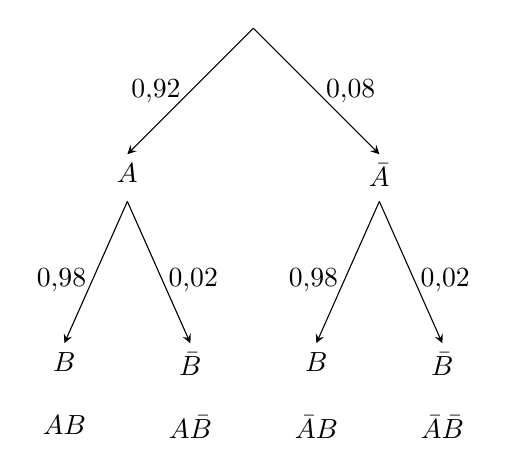
\begin{tikzpicture}[scale=.8,>=stealth]
	\coordinate [label=below:$A$](A) at (-2,-2);
	\coordinate [label=below:$\bar{A}$](B) at (2,-2);
	\coordinate [label=below:$B$](C) at (-3,-5);
	\coordinate [label=below:$\bar{B}$](D) at (-1,-5);
	\coordinate [label=below:$B$](E) at (1,-5);
	\coordinate [label=below:$\bar{B}$](F) at (3,-5);
	\draw[->](0,0)--(A);
	\draw[->](0,0)--(B);
	\draw[->](-2,-2.75)--(C);
	\draw[->](-2,-2.75)--(D);
	\draw[->](2,-2.75)--(E);
	\draw[->](2,-2.75)--(F);
	\coordinate [label=below:$AB$](G) at (-3,-6);
	\coordinate [label=below:$A\bar{B}$](H) at (-1,-6);
	\coordinate [label=below:$\bar{A} B$](I) at (1,-6);
	\coordinate [label=below:$\bar{A}\bar{B}$](J) at (3,-6);
	\draw (-1,-1) node[left] {$0{,}92$};
	\draw (1,-1) node[right] {$0{,}08$};
	\draw (-2.5,-4) node[left] {$0{,}98$};
	\draw (-1.5,-4) node[right] {$0{,}02$};
	\draw (1.5,-4) node[left] {$0{,}98$};
	\draw (2.5,-4) node[right] {$0{,}02$};
\end{tikzpicture}
\end{center}
Theo sơ đồ hình cây ta có 
\begin{itemize}
	\item Xác xuất để "Cả hai chuyến khởi hành đúng giờ" là
	$$P(AB)=0{,}92\cdot 0{,}98=0{,}9016.$$
	\item Xác suất để "Có duy nhất một trong hai chuyến bay khởi hành đúng giờ" là
	$$P(A\bar{B} \cup \bar{A}B)=0{,}92\cdot0{,}02+0{,}98\cdot 0{,}08=0{,}096.$$
	\item Xác suất để "Có ít nhất một trong hai chuyến khởi hành đúng giờ" là 
	$$P=1-P(\bar{A}\bar{B})=1-0{,}08\cdot0{,}02=0{,}9984.$$
\end{itemize}}
\end{bt}
%----
\begin{bt}%[VU NGOC HAO]%[1T9B1-4]
	Cho $A$ và $B$ là hai biến cố thoả mãn $P(A)=0{,}5 ; P(B)=0{,}7$ và $P(A \cup B)=0{,}8$.
	\begin{enumerate}
	\item [a)] Tính xác suất của các biến cố $A B, \bar{A} B$ và $\bar{A} \bar{B}$.
	\item [b)] Hai biến cố $A$ và $B$ có độc lập hay không?
	\end{enumerate}
	\loigiai{
	\begin{enumerate}
	\item [a)] Ta có $P(A \cup B)=P(A)+P(B)-P(AB) \\ \Rightarrow 
	P(AB)=P(A)+P(B)-P(A \cup B)=0,5+0,7-0,8=0,4$.\\
	$P(\bar{A} B)=P(\bar{A})P(B)=0{,}5\cdot0{,}7=0{,}35.$\\
	$P\bar{A} \bar{B}=P(\bar{A})P(\bar{B})=0{,}5\cdot0{,}3=0{,}15.$
	\item [b)] Vì $P(AB)=0,4 \neq 0,35=P(A)\cdot P(B)$ nên hai biến cố 
	$A$ và $B$ không độc lập.
	\end{enumerate}
	}
\end{bt}
\begin{bt}%[VU NGOC HAO]%[1T9K1-4]
	Vệ tinh $A$ lần lượt truyền một tin đến vệ tinh $B$ cho đến khi vệ tinh $B$ phản hồi là đã nhận được. Biết khả năng vệ tinh $B$ phản hồi đã nhận được tin ở mỗi lần $A$ gửi là độc lập với nhau và xác suất phản hồi mỗi lần đều là $0{,}4$. Sử dụng sơ đồ hình cây, tính xác suất vệ tinh $A$ phải gửi tin không quá $3$ lần.	
	\loigiai{
	\begin{center}
	\begin{tikzpicture}[font=\footnotesize, line join=round, line 
	cap=round, >=stealth,scale=1,rotate=-90]
	\path(0,0)node(a){Xác suất }
	++(2,4)node(b){ Lần 1: Nhận được}
	(a)++(2,-4)node(c){ Lần 1: Không nhận được}
	;
	\path (c)++(2,2)node(c1){Lần 2: Không nhận được}
	(c)++(2,-2)node(c2){Lần 2: Nhận được}
	;
	\path (c1)++(2,0)node(c11){Lần 3: Nhận được};
	\draw[-stealth,teal,outer sep=0,inner 
	sep=0](a.south)--(b.north) node[pos=0.5,right]{$0{,}4$};
	\draw[-stealth,teal,outer sep=0,inner 
	sep=0](a.south)--(c.north) node[pos=0.5,left]{$0{,}6$};
	\draw[-stealth,teal,outer sep=0,inner 
	sep=0](c.south)--(c1.north) node[pos=0.5,right]{$0{,}6$};
	\draw[-stealth,teal,outer sep=0,inner 
	sep=0](c.south)--(c2.north)node[pos=0.5,left]{$0{,}4$};
	\draw[-stealth,teal,outer sep=0,inner 
	sep=0](c1.south)--(c11.north)node[pos=0.5,left]{$0{,}4$};
	\end{tikzpicture}
	\end{center}	
	Vậy xác suất để vệ tinh A phải gửi tin không quá $3$ lần là 
	$0{,}4+0{,}24+0{,}144=0{,}784.$
	}
\end{bt}
%%%%
\begin{bt}%[Võ Hoàng Nghĩa]%[1T9B2-4]
	Gieo hai con xúc xăc cân đối và đồng chất. Tính xác suất của biến cố: \lq\lq Tích số chấm xuất hiện trên hai con xúc xắc chia hết cho $6$\rq\rq.
	\loigiai{
	Số phần tử của không gian mẫu: $n(\Omega)=6^2=36$.\\
	Xét biến cố A:\lq\lq Tích số chấm xuất hiện trên hai con xúc xắc chia hết cho $6$\rq\rq.\\
	Ta có\\ $A=\left\{(1;6),(2;3),(2;6),(3;2),(3;4),(3;6),(4;3),(4;6),(5;6),(6;1),(6;2),(6;3),(6;4),(6;5),(6;6)\right\} \\
	\Rightarrow n(A)=15$\\
	Vậy $P(A)=\dfrac{n(A)}{n(\Omega)}=\dfrac{15}{36}.$
	}
\end{bt}
%%%==== Câu 2===========
\begin{bt}%[Võ Hoàng Nghĩa]%[1T9K1-4]
	Một hộp có $5$ quả bóng xanh, $6$ quả bóng đỏ và $4$ quả bóng vàng có kích thước và khối lượng như nhau. Chọn ra ngẫu nhiên từ hộp $4$ quả bóng. Tính xác suất của các biến cố:\\
	A:\lq\lq Cả $4$ quả bóng lấy ra có cùng màu\rq\rq;\\
	B:\lq\lq Trong $4$ quả lấy ra có đủ $3$ màu\rq\rq.
	\loigiai{
	Xét phép thử: \lq\lq Chọn ra ngẫu nhiên từ hộp $4$ quả bóng từ một hộp chứa $15$ quả bóng\rq\rq.\\
	Số phần tử của không gian mẫu: $n(\Omega)=\mathrm{C}_{15}^4=1365.$\\
	*) Xét biến cố: A:"\\lq\lq Cả $4$ quả bóng lấy ra có cùng màu\rq\rq. Xét ba trường hợp sau:
	\begin{itemize}
	\item $4$ quả lấy ra cùng màu xanh có $\mathrm{C}_5^4$ cách.
	\item $4$ quả lấy ra cùng màu đỏ có $\mathrm{C}_6^4$ cách.
	\item $4$ quả lấy ra cùng màu vàng có $\mathrm{C}_4^4$ cách.
	\end{itemize}
	Theo quy tắc cộng ,ta có $n(A)=\mathrm{C}_5^4+\mathrm{C}_6^4+\mathrm{C}_6^4=21$ cách.\\
	Vậy xác suất để cả $4$ quả bóng lấy ra có cùng màu là: $P(A)=\dfrac{n(A)}{n(\Omega)}=\dfrac{1}{65}.$\\
	*) Xét biến cố: B:\lq\lq Trong $4$ quả lấy ra có đủ $3$ màu\rq\rq. Xét ba trường hợp sau:
	\begin{itemize}
	\item $2$ quả màu xanh, $1$ quả màu đỏ, $1$ quả màu vàng có $\mathrm{C}_5^2\cdot\mathrm{C}_6^1\cdot\mathrm{C}_4^1=240$ cách.
	\item $1$ quả màu xanh, $2$ quả màu đỏ, $1$ quả màu vàng có $\mathrm{C}_5^1\cdot\mathrm{C}_6^2\cdot\mathrm{C}_4^1=300$ cách.
	\item $1$ quả màu xanh, $1$ quả màu đỏ, $2$ quả màu vàng có $\mathrm{C}_5^1\cdot\mathrm{C}_6^1\cdot\mathrm{C}_4^2=180$ cách.
	\end{itemize}
	Theo quy tắc cộng ,ta có $n(A)=240+300+180=720$ cách.\\
	Vậy xác suất để cả $4$ quả bóng lấy ra có đủ cả ba màu là: $P(A)=\dfrac{n(A)}{n(\Omega)}=\dfrac{48}{91}.$
	}
\end{bt}
%%%==== Câu 3===========
\begin{bt}%[Võ Hoàng Nghĩa]%[1T9B1-5]
	Cường, Trọng và $6$ bạn nữ xếp ngẫu nhiên thành một hàng ngang để chụp ảnh. Tính xác suất của biến cố: "Có ít nhất một trong hai bạn Cường và Trọng đứng ở đầu hàng"
	\loigiai{
	Xét phép thử xếp ngẫu nhiên $8$ bạn, ta có số phần tử không gian mẫu $n(\Omega)=8!$\\
	Gọi $\mathrm{A}$ là biến cố: "Có ít nhất một trong hai bạn Cường và Trọng đứng ở đầu hàng"\\
	$\Rightarrow \overline{\mathrm{A}}$ là biến cố không có ai trong hai bạn Cường và Trọng đứng ở đầu hàng"
	\begin{itemize}
	\item Chọn $2$ trong $6$ bạn xếp đầu hàng có $\mathrm{A}_6^2$ cách xếp Cường và Trọng đứng ở đầu hàng
	\item Xếp $4$ bạn còn lại và hai bạn Cường và Trọng có $6!$ cách.
	\end{itemize}
	Suy ra số cách xếp cả hai bạn Cường và Trọng không đứng ở đầu hàng là: $n\left(\overline{\mathrm{A}}\right)=\mathrm{A}_6^2.6!$ cách.\\
	Vậy xác suất cần tìm là $P(A)=\dfrac{n(A)}{n(\Omega)}=\dfrac{15}{28}.$
	}
\end{bt}
%%%==== Câu 3===========
\begin{bt}%[Võ Hoàng Nghĩa]%[1T9K1-4]
	Chọn ngẫu nhiên $3$ trong $24$ đỉnh của đa giấc đều $24$ cạnh. Tính xác suất của biến cố: "$3$ đỉnh được chọn là $3$ đỉnh của một tam giác cân hoặc một tam giác vuông".
	\loigiai{
	Đa giác đều $24$ cạnh có $24$ đỉnh.\\
	Chọn $3$ đỉnh trong $24$ thì số phần tử của không gian mẫu: $n(\Omega)=\mathrm{C}_{24}^3.$\\
	Gọi $\mathrm{A}$ là biến cố "$3$ đỉnh được chọn là $3$ đỉnh của một tam giác cân hoặc một tam giác vuông"\\
	Ta có đa giác đều $24$ đỉnh nội tiếp đường tròn có $12$ đường chéo đi qua tâm. Xét hai trường hợp:
	\begin{itemize}
	\item Trường hợp 1: $3$ đỉnh được chọn là $3$ đỉnh của một một tam giác vuông hoặc cân.\\
	+) Chọn $1$ đường kính có $12$ cách.\\
	+) Chọn $1$ đỉnh trong $22$ đỉnh còn lại có $22$ cách.\\
	Vậy trường hợp này có $12.22=264$ (tam giác vuông hoặc cân).
	\item Trường hợp 2: $3$ đỉnh được chọn là $3$ đỉnh của một tam giác cân\\
	+) Chọn $1$ đỉnh trong $2$ đỉnh của $1$ đường kính có $2$ cách.\\
	+) Mỗi đường kính chia đa giác thành hai miền, mỗi miền có $11$ đỉnh.\\
	+) Chọn $1$ đỉnh thuộc miền thứ nhất thì tương ứng có $1$ đỉnh thuộc miền thứ hai để $3$ đỉnh được lập thành tam giác cân.\\
	Vậy trường hợp này có $12.2.11=264$ (tam giác cân)
	\end{itemize}
	Suy ra $n(\mathrm{A})=528.$
	Vậy Vậy xác suất cần tìm là $P(A)=\dfrac{n(A)}{n(\Omega)}=\dfrac{6}{23}.$
	}
\end{bt}
%%%==== Câu 4===========
\begin{bt}%[Võ Hoàng Nghĩa]%[1T9K1-4]
	Chọn ngẫu nhiên một số từ tập hợp các số tự nhiên có $3$ chữ số. Tính xác suất của các biến cố:\\
	A:"Số được chọn chia hết cho $2$ hoặc $7$."\\
	B:"Số được chọn có tổng các chữ số là số chẳn".
	\loigiai{
	Số tự nhiên của $3$ chữ số có dạng $x=\overline{abc}$, với $a\neq 0; a,b,c \in \left\{0;1;2;\cdots ; 9\right\}$\\
	+) $a$ có $9$ cách chọn.\\
	+) $b$ có $10$ cách chọn.\\
	+) $c$ có $10$ cách chọn.\\
	Khi đó số phần tử của không gian mẫu là $n(\Omega)=9.10.10=900$ (số).\\
	Xét biến cố: A:"Số được chọn chia hết cho $2$ hoặc $7$."
	\begin{itemize}
	\item Số được chọn chia hết cho $2$.\\
	Khi đó ta có thêm điều kiện $c \in \left\{0;2;4;6;8\right\}\Rightarrow c$ có $5$ cách chọn.\\
	+) $a$ có $9$ cách chọn.\\
	+) $b$ có $10$ cách chọn.\\
	Suy ra trường hợp này có $5.9.10=450$ (số)
	\item Số được chọn chia hết cho $7$
	Khi đó để $x \hspace{0.1cm}\vdots\hspace{0.1cm} 7$ thì $\left(c+3b+2a\right) \hspace{0.1cm}\vdots\hspace{0.1cm} 7$\\
	Suy ra $x \in \left\{ 112; 119; \cdots 994\right\}$ và trường hợp này có $\dfrac{994-112}{7}+1=127$ (số).\\
	\end{itemize}
	Theo quy tắc cộng, ta có: $n(A)=450+127=577$ (số).\\
	Vậy $P(A)=\dfrac{n(A)}{n(\Omega)}=\dfrac{577}{900}.$
	}
\end{bt}
%%%==== Câu 5===========
\begin{bt}%[Võ Hoàng Nghĩa]%[1T9K1-5]
	Cho hai giống cá kiếm mắt đen thuần chủng và mắt đỏ thuần chủng giao phối với nhau được $\mathrm{F1}$ toàn cá kiếm mắt đen. Lại cho cá $\mathrm{F1}$ giao phối với nhau lại được cá con mới. Chọn ra ngẫu nhiên $2$ con trong đàn cá con mới. Ước lượng xác suất của biến cố:"Có ít nhất $1$ con cá mắt đen trong $2$ con cá đó."
	\loigiai{
	Vì $\mathrm{F1}$ toàn cá kiếm mắt đen nên mắt đen là tính trạng trội, mắt đỏ là tính trạng lặn.\\
	Gọi $\mathrm{A, a}$ lần lượt là gen mang tính trạng trội và lặn.\\
	\begin{eqnarray*}
	\mathrm{P}&:&AA\hspace{1cm} \times \hspace{0.75cm}aa\\
	\mathrm{Gp}&:&A\hspace{1cm} \times \hspace{1cm}a\\
	\mathrm{F1}&:& \hspace{1.5cm}Aa.	
	\end{eqnarray*}	
	\begin{eqnarray*}
	\mathrm{F1} \times \mathrm{F1} &:&Aa\hspace{1cm} \times \hspace{1cm}Aa\\
	\mathrm{Gp}&:&A,a\hspace{1cm} \times \hspace{1cm}A,a\\
	\mathrm{F2}&:& 1AA,\hspace{0.1cm}2Aa,\hspace{0.1cm}1aa.
	\end{eqnarray*}
	Vậy đàn cá con mới gồm $3$ con mắt đen và $1$ con mắt đỏ.\\
	Do đó xác suất để chọn được ít nhất $1$ con cá mắt đen là $100\%$
	}
\end{bt}